\subsection{Module 8: Các chức năng về nhắn tin cho chủ nhà}
\subsubsection{User stories}
\begin{itemize}
    \item Chủ nhà có thể nhận và đọc tin nhắn từ khách thuê.
    \item Chủ nhà có thể  phản hồi cho khách thuê.
    \item Chủ nhà có thể xoá tin nhắn.
\end{itemize}


% ########################################################
\begin{figure}[!h]
	\centering
	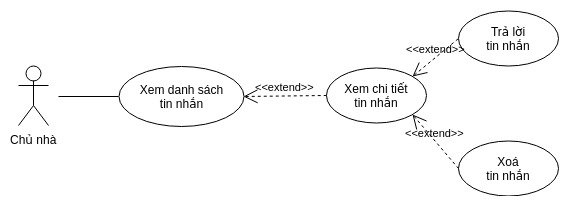
\includegraphics[width=\textwidth]{parts/Cuong/images/module5c.jpg}
	\caption{Lược đồ use case của module 5c: Các chức năng về nhắn tin cho chủ nhà}
\end{figure}

% ########################################################
\subsubsection{Các use case chi tiết}
\subsubsubsection{Xem danh sách tin nhắn}
\begin{usecase}
    \usecasename{Xem danh sách tin nhắn}
	\actor{Chủ nhà}
	\describe{Chủ nhà xem danh sách tất cả tin nhắn đã nhận từ các khách thuê.}
	\creators{Văn Tiến Cường}{Văn Tiến Cường}
	\datecreated{22/03/2019}{30/03/2019}
	\precond{Chủ nhà đã đăng nhập thành công}
	\postcond{Hệ thổng hiển thị danh sách các tin nhắn được gửi cho chủ nhà}
	\normalflow
	\begin{enumerate}
		\item Chủ nhà chọn mục \textbf{Tin nhắn}.
        \item Hệ thống hiện ra danh sách tin nhắn, người gửi, chủ đề, trạng thái đặt phòng của người khách đó.
	\end{enumerate} \\ \hline
	
	\noalternative
	\noexception
\end{usecase}

\subsubsubsection{Xem chi tiết tin nhắn}
\begin{usecase}
    \usecasename{Xem chi tiết tin nhắn}
    \actor{Chủ nhà}
    \describe{Chủ nhà xem chi tiết một tin nhắn trong danh sách tin nhắn đã gửi cho mình}
    \creators{Văn Tiến Cường}{Văn Tiến Cường}
	\datecreated{22/03/2019}{30/03/2019}
    \precond{Chủ nhà đang xem danh sách tin nhắn}
    \postcond{Hiện thông tin chi tiết về tin nhắn được chủ nhà chọn xem}
    
    \normalflow
	\begin{enumerate}
        \item Chủ nhà chọn một tin nhắn trong danh sách tin nhắn.
        \item Hệ thống hiển thị tin nhắn cho chủ nhà, gồm các trường \textbf{Người gửi}, \textbf{Thời gian gửi}, \textbf{Chủ đề}, \textbf{Nội dung tin nhắn}, \textbf{Trạng thái đặt phòng}.
    \end{enumerate} \\ \hline
        
    \noalternative
    \noexception
\end{usecase}

\subsubsubsection{Trả lời tin nhắn}
\begin{usecase}
    \actor{Chủ nhà}
    \describe{Chủ nhà trả lời cho một tin nhắn đã gửi cho mình}
    \creators{Văn Tiến Cường}{Văn Tiến Cường}
	\datecreated{22/03/2019}{30/03/2019}
    \precond{Chủ nhà đang xem chi tiết một tin nhắn nào đó}
    \postcond{Hệ thống gủi tin nhắn phản hồi tới cho khách thuê và thông báo thành công}

    \normalflow
	\begin{enumerate}
        \item Chủ nhà chọn nút \textbf{Trả lời}.
        \item Chủ nhà nhập nội dung phản hồi.
        \item Chủ nhà chọn nút \textbf{Gửi}.
        \item Hệ thống thông báo tin nhắn gửi thành công.
    \end{enumerate} \\ \hline
        
    \noalternative
    
    \exception
    \begin{enumerate}
        \alt{3a} Chủ nhà chọn \textbf{Huỷ}. Hệ thống sẽ huỷ tin nhắn hiện tại và trở về hiển thị tin nhắn chi tiết.
    \end{enumerate} \\ \hline
\end{usecase}


\subsubsubsection{Xoá tin nhắn}
\begin{usecase}
    \actor{Chủ nhà}
    \describe{Chủ nhà xoá một tin nhắn đã chọn}
    \creators{Văn Tiến Cường}{Văn Tiến Cường}
	\datecreated{22/03/2019}{30/03/2019}
    \precond{Chủ nhà đang xem chi tiết một tin nhắn nào đó}
    \postcond{Tin nhắn được chọn bị xoá và hệ thống hiện thông báo xoá thành công}
    
    \normalflow
    \begin{enumerate}
		\item Chủ nhà chọn nút \textbf{Xoá}.
        \item Hệ thống yêu cầu xác nhận xoá.
        \item Chủ nhà chọn \textbf{Đồng ý}.
        \item Hệ thống thông báo xoá tin nhắn thành công.
	\end{enumerate} \\ \hline
	
	\noalternative
    
    \exception
    \begin{enumerate}
        \alt{3a} Chủ nhà chọn \textbf{Huỷ}. Hệ thống sẽ huỷ tin nhắn hiện tại và trở về hiển thị tin nhắn chi tiết.
    \end{enumerate} \\ \hline
\end{usecase}